\vspace{-0.01in}
\section{Gemmini Generator}\label{sec:generator}
% \vspace{-0.05in}

% Gemmini is an open-source, full-stack generator of DNN accelerators, spanning across different architectures, programming interfaces, and system integration options. At the hardware level, Gemmini's architectural template is flexible enough to support a diverse set of numerical and structural microarchitecture parameters.
% In addition, Gemmini also produces software binaries tuned for each created hardware instance, either through a push-button programming interface via the ONNX Runtime~\cite{onnxruntime} or a low-level, Gemmini-provided Application Programming Interface (API) that is portable across Gemmini-generated accelerators.
% Programmers can target the provided API if they wish to write their own applications or create their own kernels.
% Finally, Gemmini generates not only accelerators, but full SoCs which can run real-world software stacks, including operating systems, during design space exploration. This enables architects to accurately evaluate the impact of the full SoC and software stack on efficiency and performance.

Gemmini is an open-source, full-stack generator of DNN accelerators, spanning across different hardware architectures, programming interfaces, and system integration options.
With Gemmini, users can generate everything from low-power edge accelerators to high-performance cloud accelerators equipped with out-of-order CPUs. Users can then investigate how the hardware, SoC, OS, and software overhead interact to affect overall performance and efficiency.

\subsection{Architectural Template}
\label{ssec:arch}

\begin{figure}[t]
    \centering
    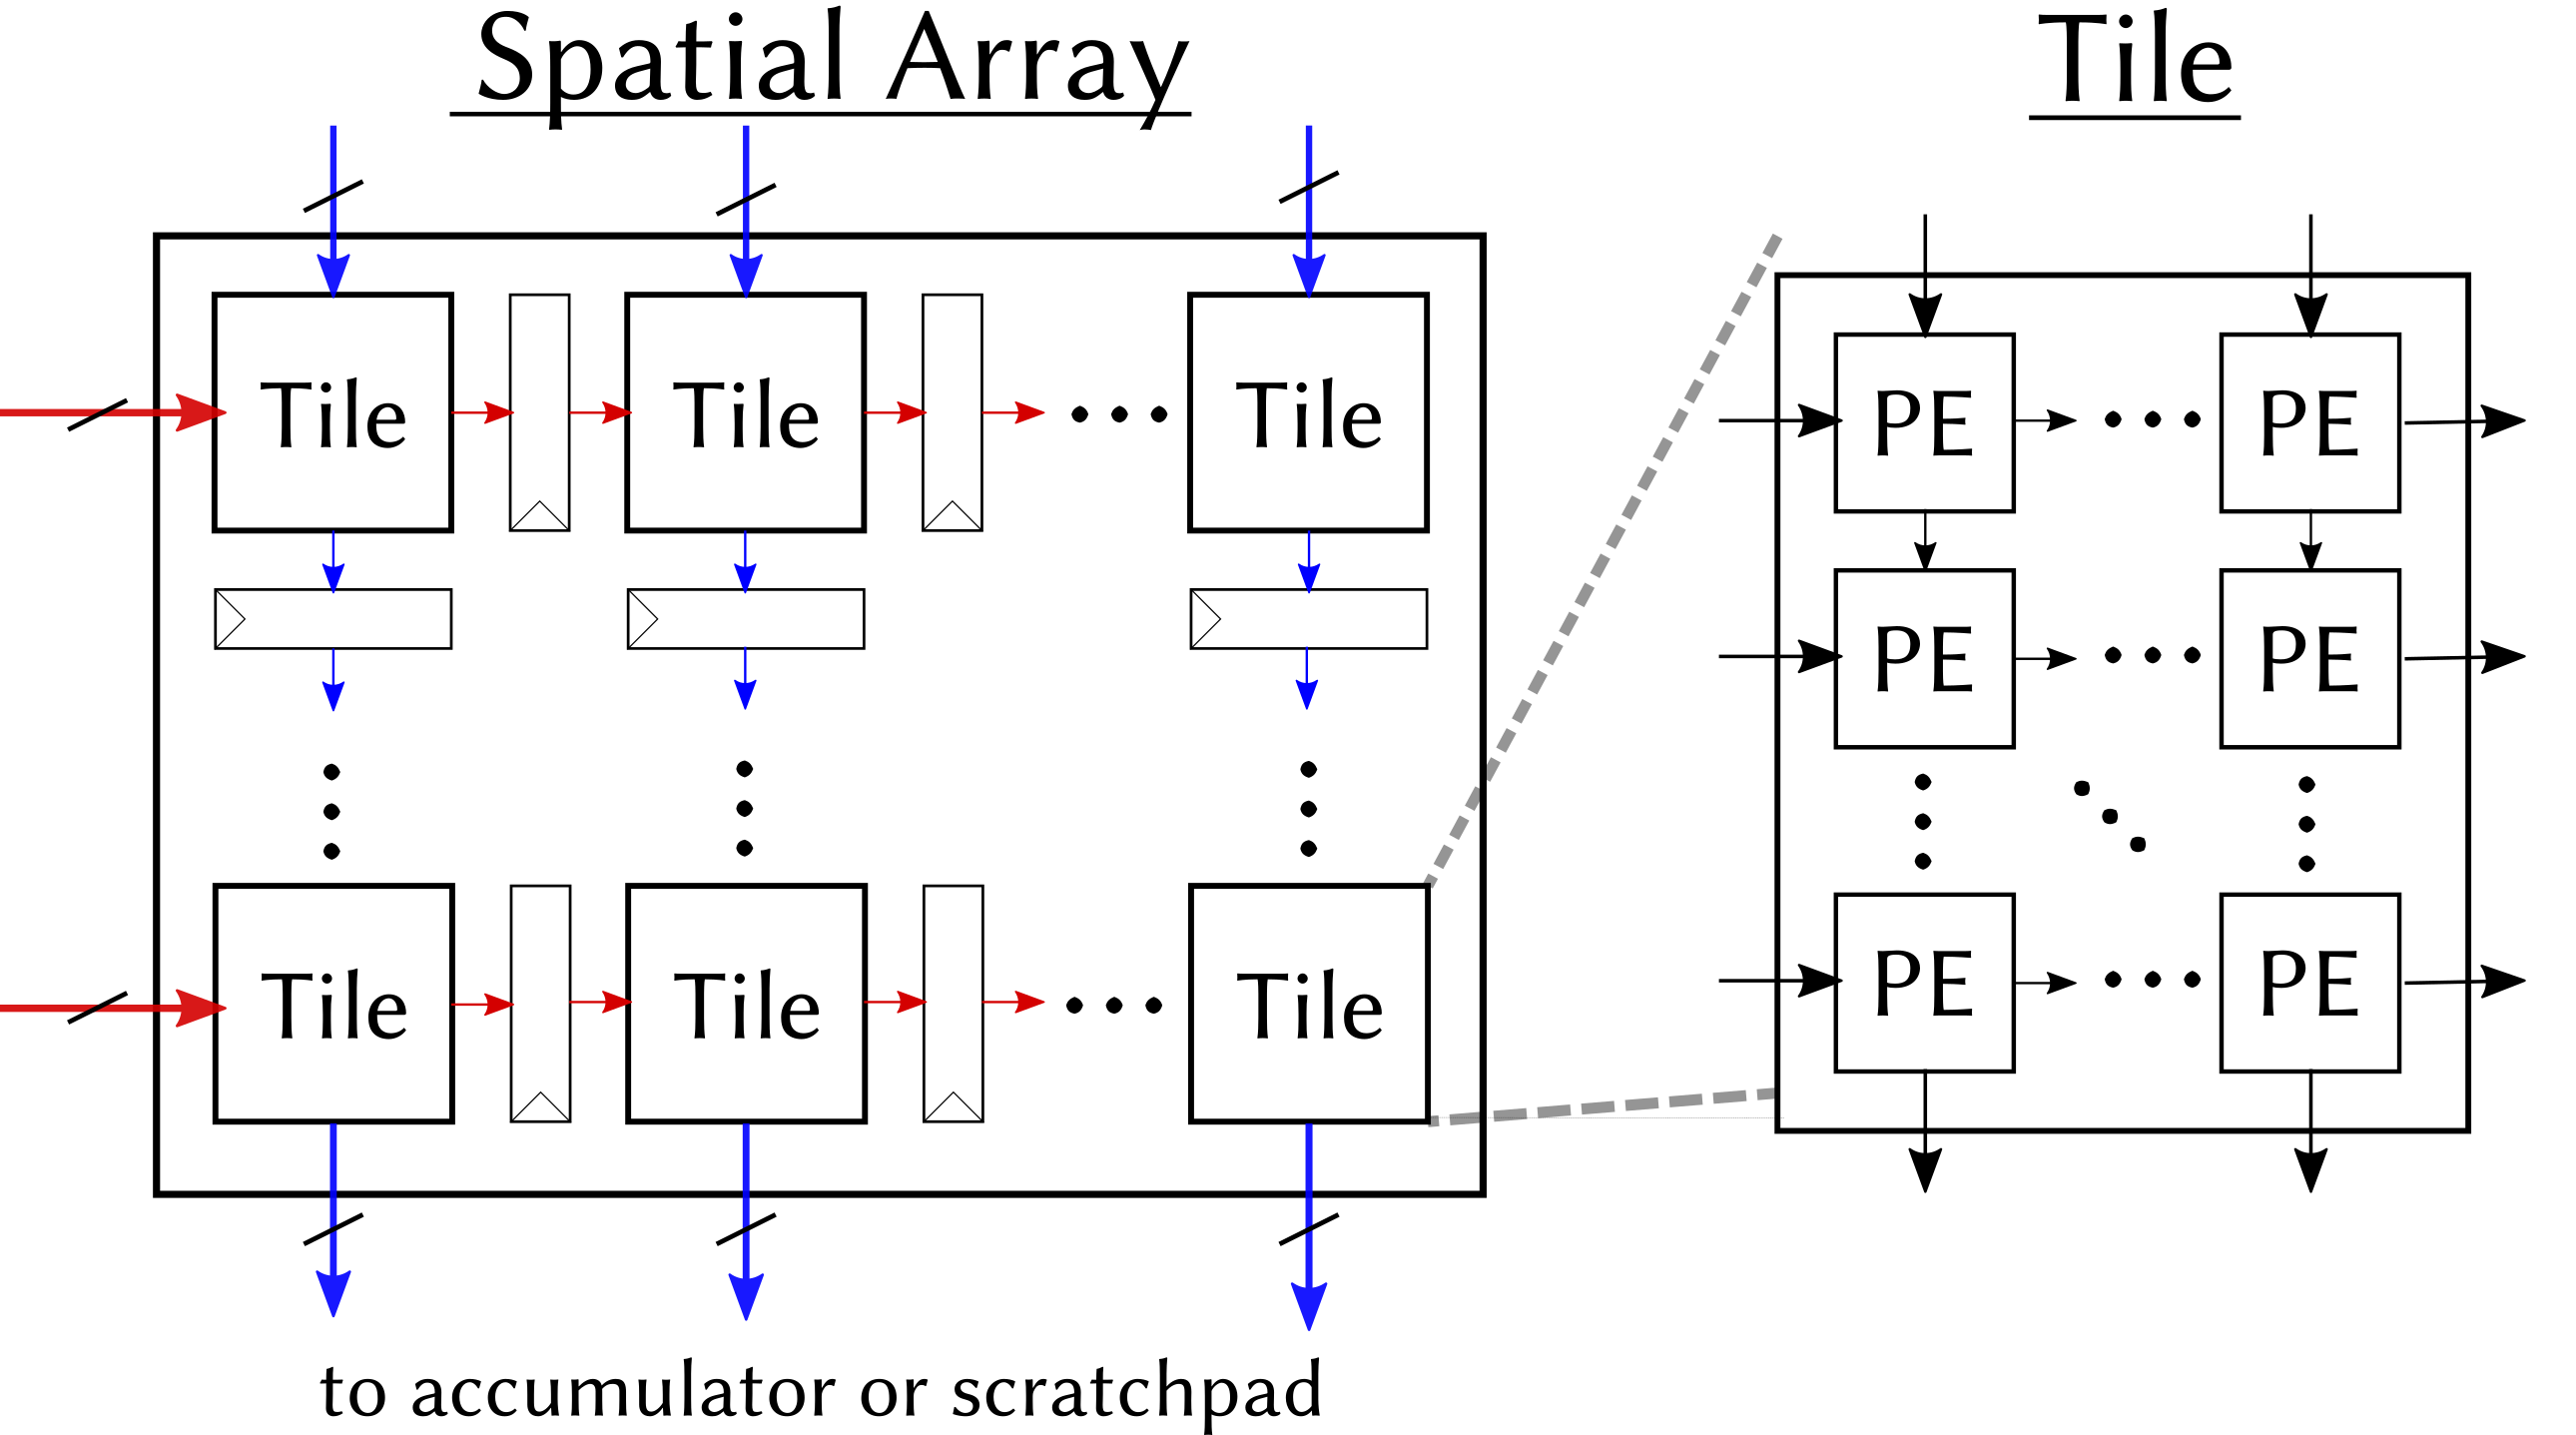
\includegraphics[width=0.85\linewidth]{fig/systolic_arch_detail3.png}
    \caption{Microarchitecture of Gemmini's two-level spatial array.} % The spatial array is composed of \textit{tiles}, connected via explicit, pipelined registers. Each tile can be further broken down into an array of \textit{Processing Elements (PEs)}, connected by a fully combinational grid.}
    \label{fig:systolic_arch}
    \vspace{-0.2in}
\end{figure}

Figure~\ref{fig:arch-template} illustrates Gemmini's architectural template.
The central unit in Gemmini's architectural template is a spatial architecture with spatially distributed processing elements (PEs), each of which performs dot products and accumulations.
The spatial array reads data from a local, explicitly managed scratchpad of banked SRAMs, while it writes results to a local accumulator storage with a higher bitwidth than the inputs.
Gemmini also supports other commonly-used DNN kernels, \textit{e.g.}, pooling, non-linear activations (ReLU or ReLU6), and matrix-scalar multiplications, through a set of configurable, peripheral circuitry.
Gemmini-generated accelerators can also be integrated with a RISC-V host CPU
to program and configure accelerators.

% \subsubsection{Spatial Array}

We design Gemmini's spatial array with a two-level hierarchy to provide a flexible template for different microarchitecture structures, as demonstrated in Figure~\ref{fig:systolic_arch}.
The spatial array is first composed of \textit{tiles}, where tiles are connected via explicit pipeline registers.
Each of the individual tiles can be further broken down into an array of PEs, where PEs in the same tile are connected combinationally without pipeline registers.
Each PE performs a single multiply-accumulate (MAC) operation every cycle, using either the weight- or the output-stationary dataflow.
The tiles are composed of rectangular arrays of PEs, where PEs in the same tile are connected combinationally with no pipeline registers in between them. The spatial array, likewise, is composed of a rectangular array of tiles, but each tile \textit{does} have pipeline registers between it and its neighbors.
Every PE and every tile shares inputs and outputs only with its adjacent neighbors.

Figure~\ref{fig:nvdla-vs-tpu-comparison} illustrates how Gemmini's two-level hierarchy provides the flexibility to support anything from fully-pipelined TPU-like architectures to NVDLA-like parallel vector engines where PEs are combinationally joined together to form MAC reduction trees, or any other design points in between these two extremes. We synthesized both designs with 256 PEs. We found that the TPU-like design achieves a 2.7x higher maximum frequency, due to its shorter MAC chains, but consumes 1.8x as much area as the NVDLA-like design, and 3.0x as much power, due to its pipeline registers. With Gemmini, designers can explore such footprint vs. scalability trade-offs across different accelerator designs.

\begin{figure}[t]
\centering
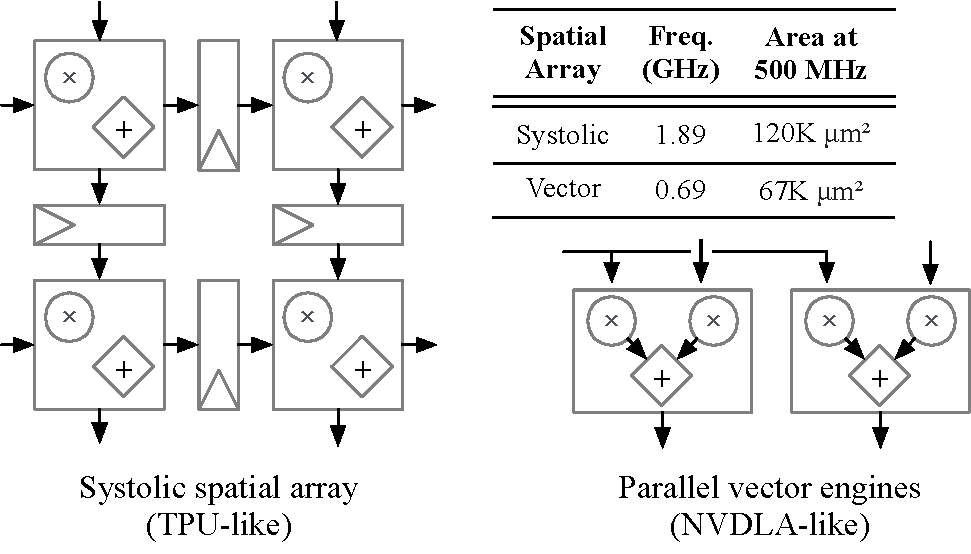
\includegraphics[width=\linewidth]{fig/Systolic-vs-NVDLA-smaller2.pdf}
\vspace{-0.2in}
\caption{Examples of two different spatial architectures generated by Gemmini. Both perform four multiply-accumulates per cycle though with different connectivities between multiply-and-accumulate units.}
\label{fig:nvdla-vs-tpu-comparison}
\vspace{-0.2in}
\end{figure}

% \begin{figure}[t]
% \centering
% \begin{subfigure}[b]{0.4\linewidth}
%     \centering
%     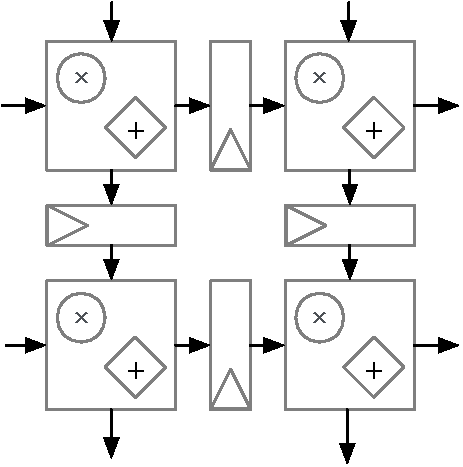
\includegraphics[width=\linewidth]{fig/tpu-like}
%     \caption{TPU-like spatial array with systolic processing.}
%     \label{fig:tpu-like}
% \end{subfigure}
% \hspace{0.05\linewidth}
% \begin{subfigure}[b]{0.45\linewidth}
%     \centering
%     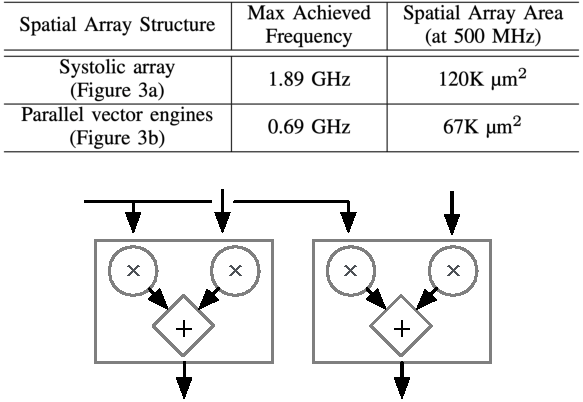
\includegraphics[width=\linewidth]{fig/NVDLA-smaller.pdf}
%     \caption{NVDLA-like spatial array with parallel vector engines.}
%     \label{fig:nvdla-like}
% \end{subfigure}
% \caption{Examples of two different spatial architectures generated by Gemmini. Both perform four multiply-accumulates per cycle though with different connectivities between multiply-and-accumulate units.}
% \vspace{-0.1in}
% \end{figure}

% These kinds of performance vs. footprint vs. scalability trade-offs must be decided by architects for any accelerator they design. Gemmini provides a unified framework with which they can generate and evaluate different architectures, making the design space exploration process simpler and easier.

% Table~\ref{tab:tpu-vs-nvdla} shows the maximum achieved frequency and area footprint of these two designs synthesized with Intel $22nm$ FinFET process.
% We notice that the systolic design achieves a 2.7$\times$ higher frequency than the parallel vector engines, as the extra pipeline registers greatly reduced the critical path lengths, demonstrating better scalability especially for larger array dimensions.
% %The is not unexpected, as systolic arrays are known to have strong scalability during physical design~\cite{}.
% At the same time, the extra pipeline registers also add significant area overhead of the systolic array, so that it consumes 1.8$\times$ more area compared to the parallel vector engines, and 3.0$\times$ as much power.

%These kinds of performance vs. footprint vs. scalability trade-offs must be decided by architects for any accelerator they design. Gemmini provides a unified framework with which they can generate and evaluate different architectures, making the design space exploration process simpler and easier.

% Gemmini supports this microarchitectural variation naturally by representing the spatial array as a two-level hierarchy. The inner dimension, which we call \textit{tiles}, is composed of combinationally-connected PE, where each PE performs a single multiply-accumulate operation per cycle. The outer dimension, which is the spatial array itself, is composed of tiles with pipeline registers between them. By tuning the sizes of the tiles within an array, architects can group individual PEs under the same combinational mesh, where they can be merged into dot-product reduction trees. Alternatively, limiting each tile to a size of only one PE produces a totally systolic design.

%\subsubsection{Parameters}

% \hl{Gemmini supports a large number of parameters, allowing a high degree of customization over the compute characteristics, memory capacity, and SoC-level characteristics of any accelerator that is generated. The most relevant parameters, described in Table~\mbox{\ref{tab:parameter-table}}, configure all parts of the compute stack, from the dataflow of the spatial array to the cache hierarchy of the host CPU and the main memory. For example, we can configure the datatype of the PEs to signed integers, unsigned integers, or floats, of any size defined by the user.}

% \begin{table}[t]
% \centering
% \begin{tabular}{l|c|c}
% \hline
% \makecell{Spatial Array Structure} & \makecell{Max Achieved\\Frequency} & \makecell{Spatial Array Area \\ (at 500 MHz)} \\ \hline\hline
% \makecell{Systolic array\\(Figure~\ref{fig:tpu-like})}          & 1.89 GHz               & 120K {\textmu}m$^2$       \\ \hline
% \makecell{Parallel vector engines\\(Figure~\ref{fig:nvdla-like})} & 0.69 GHz                & 67K {\textmu}m$^2$        \\ \hline
% \end{tabular}
% \caption{Maximum frequency and area footprint for two different Gemmini-generated spatial array architectures.}
% \vspace{-0.1in}
% \label{tab:tpu-vs-nvdla}
% \vspace{-0.1in}
% \end{table}

% \begin{table}[t]
% \begin{tabular}{ c | l | c }
% \hline
% \textbf{Category} & \textbf{Parameter} &  \textbf{Recommended Range} \\  
% \hline
% \hline
% \multirow{5}{*}{\makecell{Spatial\\Array}} & Mesh Rows & 1--256 \\
% & Mesh Columns & 1--256 \\
% & Tile Rows  & 1--256  \\
% & Tile Columns  & 1--256  \\
% & Dataflow & \makecell{Weight/Output stationary,\\or both} \\
% \hline
% \multirow{4}{*}{\makecell{\makecell{Accelerator\\Memory}}} & Scratchpad Capacity & 256 bytes--16 MB \\
% & Accumulator Capacity  & 256 bytes--8 MB  \\
% & Scratchpad Banks  & 1--4 \\
% & Accumulator Banks  & 1--4 \\
% \hline
% \multirow{3}{*}{\makecell{\makecell{Execution\\Schedule}}} & ROB Entries & 4--128 \\
% & Load Queue Entries & 2--128 \\
% & Store Queue Entries & 2--128\\
% & Execute Queue Entries & 4--128 \\
% \hline
% \multirow{4}{*}{\makecell{\makecell{Controller}}} & PE Latency & 0--4 cycles \\
% & DMA Bus Width & 64--256 bits \\
% & DMA Block Size & 32--64 bytes \\
% & TLB Entries & 2--64 \\
% \hline
% \multirow{4}{*}{\makecell{\makecell{Datatypes}}} & Datatype & SInt/UInt/Float/User-defined \\
% & Input Bitwidth & 8--32 bits \\
% & Output Bitwidth & 8--32 bits \\
% & Accumulator Bitwidth & 16--64 bits \\
% \hline
% \multirow{3}{*}{\makecell{\makecell{Operators}}} & Multiply by Scalar & Present/Not \\
% & Transposer & Present/Not \\
% & Pooling & Present/Not \\
% & Im2col & Present/Not \\
% \hline
% \multirow{6}{*}{\makecell{\makecell{System}}} & Host Processor\footnote{Each host processor has a long list of potential parameters associated with it} & Rocket, BOOM \\
% & Number of Cores & 1-64 \\
% & Number of Accelerators & 0-Number of Cores \\
% & Shared L2 Cache Size & 256 KB -- 16 MB \\
% & Peripherals & UART, GPIO, SPI, JTAG, etc. \\
% & IO Models & \makecell{Network, DDR3, Block Device\\Latency-Bandwidth pipeline} \\ 
% \hline
% \end{tabular}
% \caption{Gemmini hardware configurable parameters. For the integer ranges, all power-of-2 values between the maximum and minimum are permitted. All parameters are independent of each other, and the size of the total search space is the cross-product of all possible parameter values. \textcolor{red}{HASAN: Cut table 3 in half.}}
% \label{tab:parameter-table}
% \end{table}

% \hl{\textbf{Optional compute blocks:} Peripheral compute blocks also exist to support non-linear activation functions, max-pooling, transpositions, and im2col. These blocks can be optionally left out of the generator to save area and power consumption for workloads that do not require them. The im2col block allows us to support both convolutions and matrix multiplications efficiently with the same spatial array.} \textcolor{red}{Should we mention the optional compute blocks?}

% \hl{The presence or absence of these blocks can significantly affect the performance and memory requirements of Gemmini applications at runtime. For example, if the im2col module is \textit{not} instantiated, then the Gemmini-generated accelerator will not be able to perform arbitrary convolutions directly on the input data. Instead, it will first map those convolutions to matrix multiplications through the im2col~\mbox{\cite{chetlur2014cudnn}} operation, which runs on the CPU and duplicates data, causing a significant memory expansion. Those im2col-ed buffers are then fed into the Gemmini-generated accelerator's local scratchpad increasing memory storage requirements and saturating the memory bandwidth.}

% \hl{
% However, if the im2col block \textit{is} instantiated, then Gemmini will instead run a seven-nested convolution loop directly, without requiring the host CPU to shuffle and duplicate data. Instead, the im2col module within the accelerator will repeatedly fetch the same pieces of data and feed them multiple times into the spatial array. Therefore, the duplication essentially happens \textit{in time} in the interface between the local scratchpad and the spatial array, rather than happening \textit{in space} in local or main memory.
% We demonstrate the performance impact of using the im2col module over running im2col on the host CPU in Section~\mbox{\ref{sec:evaluation}}.
% }

% \subsubsection{Im2Col}

% \hl{
% We demonstrate the operation of the im2col block in Figure~\mbox{\ref{fig:im2col}}. The im2col module is essentially an address generator which repeatedly fetches the same scratchpad entries across different matrix multiplications. The programmer only specifies the dimensions of the convolution operator (e.g. kernel width, image height, etc.) and the im2col block then generates all the (potentially non-contiguous) scratchpad addresses necessary to perform a convolution on the accelerator.
% }

% \begin{figure}[h]
%     \vspace{-0.2cm}
%     \centering
%     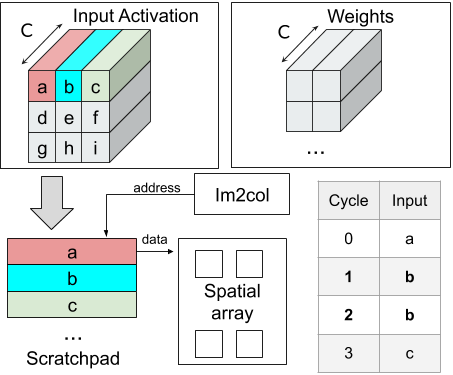
\includegraphics[width=0.7\linewidth]{fig/im2col.png}
%     \caption{Operation of im2col block, showing when different entries in the scratchpad are fed into the spatial array. Notice how the same row of the input activations, $b$, is fed into the spatial array multiple times. In cycle 1, $b$ is fed into the PEs on the first row of the spatial array, and in cycle 2, $b$ is fed into the PEs on the second row of the spatial array.}
%     \label{fig:im2col}
%     \vspace{-0.15in}
% \end{figure}

\subsection{Programming Support}
\label{software}

The Gemmini generator produces not just a hardware stack, but also a tuned software stack, boosting developers' productivity as they explore different hardware instantiations.
Specifically, Gemmini provides a multi-level software flow to support different programming scenarios.
At the \textit{high level}, Gemmini contains a push-button software flow which reads DNN descriptions in the ONNX file format
% ~\cite{onnx}
and generates software binaries that will run them, mapping as many kernels as possible onto the Gemmini-generated accelerator. Alternatively, at the \textit{low level}, the generated accelerator can also be programmed through C/C++ APIs, with tuned functions for common DNN kernels. These functions must be tuned differently for different hardware instantiations in order to achieve high performance, based on scratchpad sizes and other parameters. Therefore, every time a new accelerator is produced, Gemmini also generates an accompanying header file containing various parameters, \textit{e.g.} the dimensions of the spatial array, the dataflows supported, and the compute blocks that are included (such as pooling, im2col, or transposition blocks).

\begin{figure}[t]
    \centering
    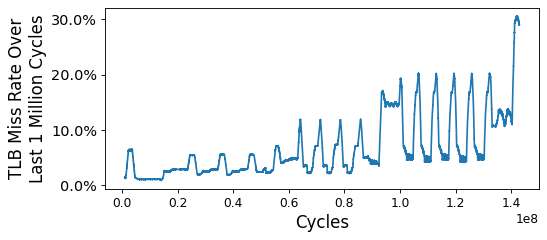
\includegraphics[width=\linewidth]{fig/tlb_hit_rate_running.png}
    \caption{TLB miss rate over a full ResNet50 inference, profiled on a Gemmini-generated accelerator.}
    \label{fig:tlb_hit_rate}
    \vspace{-0.2in}
\end{figure}

\textbf{Data Staging and Mapping:}
At runtime, based on the dimensions of a layer's inputs, and the hardware parameters of the accelerator instantiation, Gemmini uses heuristics to maximize the amount of data moved into the scratchpad per iteration.
Gemmini calculates loop tile sizes at runtime, and these tile sizes determine when and how much data is moved between DRAM, L2, and scratchpad during the execution of our tiled matrix multiplication, convolution, residual-addition, etc. kernels.
If the programmer wishes, the low-level API also allows them to manually set tile-sizes for each kernel.
% This runtime tuning is transparent to the programmer so that they can call the same DNN kernel functions to offload tasks onto different Gemmini-generated accelerators even if they were parameterized differently, without any porting or re-programming effort required.

\textbf{Virtual Memory Support:}
In addition to the programming interface, Gemmini also makes it easier to program accelerators by providing virtual memory support. This is useful for programmers who wish to avoid manual address translations as well as for researchers who wish to investigate virtual memory support in modern accelerators.
Gemmini also enables users to co-design and profile their own virtual address translation system. For example, Figure~\ref{fig:tlb_hit_rate} shows the miss rate of an example accelerator's local TLB profiled on Gemmini. As we can see, the miss rate occasionally climbs to 20-30\% of recent requests, due to the tiled nature of DNN workloads, which is orders-of-magnitude greater than the TLB miss rates recorded in prior CPU non-DNN benchmarks~\cite{lustig2013tlb}.
Later, in Section~\ref{virtual-memory-case-study}, we use Gemmini to co-design a virtual address translation system which achieves near-maximum end-to-end performance on accelerated DNN workloads, with only a few TLB entries in total.

\subsection{System Support}
\label{system}

% Gemmini supports full SoC integration, as well as evaluation on a realistic software stack including OS overheads, through its integration with the Chipyard SoC framework~\cite{chipyard}.
% Using Chipyard, Gemmini parameterizes not only the accelerator itself, but also the host CPU, memory interconnects, main memory cache hierarchy, and other system-level parameters.
% These components can be elaborated, interconnected, evaluated with a real software stack including operating-system overheads, and pushed through VLSI implementation flows~\cite{Hammer}, all within the unified Chipyard environment. 
% Cycle-exact simulations can run on the FPGA-accelerated FireSim~\cite{karandikar2018firesim} platform, even when evaluating large, complex SoCs running entire operating systems alongside compute-intensive workloads.

%\subsubsection{SoC Parameters}

%Gemmini provides a number of SoC parameters which modify the SoC outside the accelerator itself.
%We describe here some of these parameters and their potential impact on performance and efficiency.

%\textbf{Host CPU (Single- and Multi-Core):} 
Gemmini allows architects to integrate RISC-V CPUs % which supports the RoCC interface~\cite{Rocket-RISCV-2016}
with Gemmini-generated accelerators in the Chipyard~\cite{chipyard} framework.
These can range from simple, in-order microcontrollers which are not expected to do much more than IO management, all the way up to out-of-order, high-performance, server-class CPUs that may be running multiple compute-intensive applications even as they are sending commands to the Gemmini-generated accelerator.
% As DNN models evolve, some host CPUs may be required to complete execute operations and control flow that are not supported by Gemmini, increasing their impact upon overall performance.
SoCs can also be configured to host \textit{multiple} host CPUs and Gemmini-generated accelerators, which can each operate on different tasks in parallel with each other. Figure~\ref{fig:contention-soc} is one example of a dual-core system, where each CPU has its own Gemmini-generated accelerator.
Additional SoC-level parameters include bus widths between accelerators and host CPUs, as well as the size, associativity and hierarchy of the caches in the multicore, multicache memory system. Later, in Section~\ref{cache-contention}, we show how these parameters can be tuned, based on the computational characteristics of DNNs, to improve performance by over~8\%.

\begin{figure}[t]
     \centering
     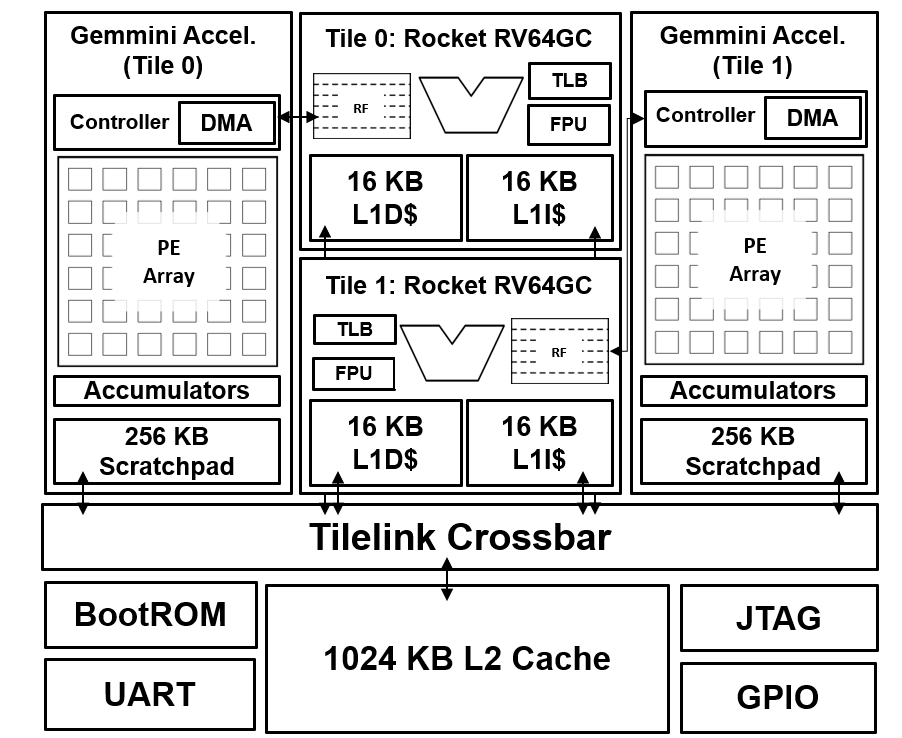
\includegraphics[width=0.75\linewidth]{fig/contention-soc.png}
     \caption{Example dual-core SoC with a Gemmini accelerator attached to each CPU, as well as a shared L2 cache and standard peripherals.}
     \label{fig:contention-soc}
     \vspace{-0.2in}
 \end{figure}

RISC-V-based full SoC integration also enables deep software-stack support, such that Gemmini-generated accelerators can easily be evaluated running the full software stack up to and including the operating system itself. This enables early exploration of accelerated workloads in a realistic environment where context switches, page table evictions, and other unexpected events can happen at any time. These unexpected events can uncover bugs and inefficiencies that a ``baremetal'' environment would not bring to the surface. For example, our experience of running Linux while offloading DNN kernels to a Gemmini-generated accelerator uncovered a non-deterministic deadlock that would only occur if context switches happened at very particular, inopportune times.
Running on a full software stack with an OS also uncovered certain bugs where Gemmini read from certain regions of physical memory without the proper permissions. On a ``baremetal'' environment, these violations were silently ignored.

